Previously, we found the splitting field for $x^3-2,$ $K=\Q(\sqrt[3]{2}, \omega)$, and we calculated $\Gal{\Q(\sqrt[3]{2}, \omega)/\Q}$. We also looked at subfields of $\Q(\sqrt[3]{2}, \omega)$:

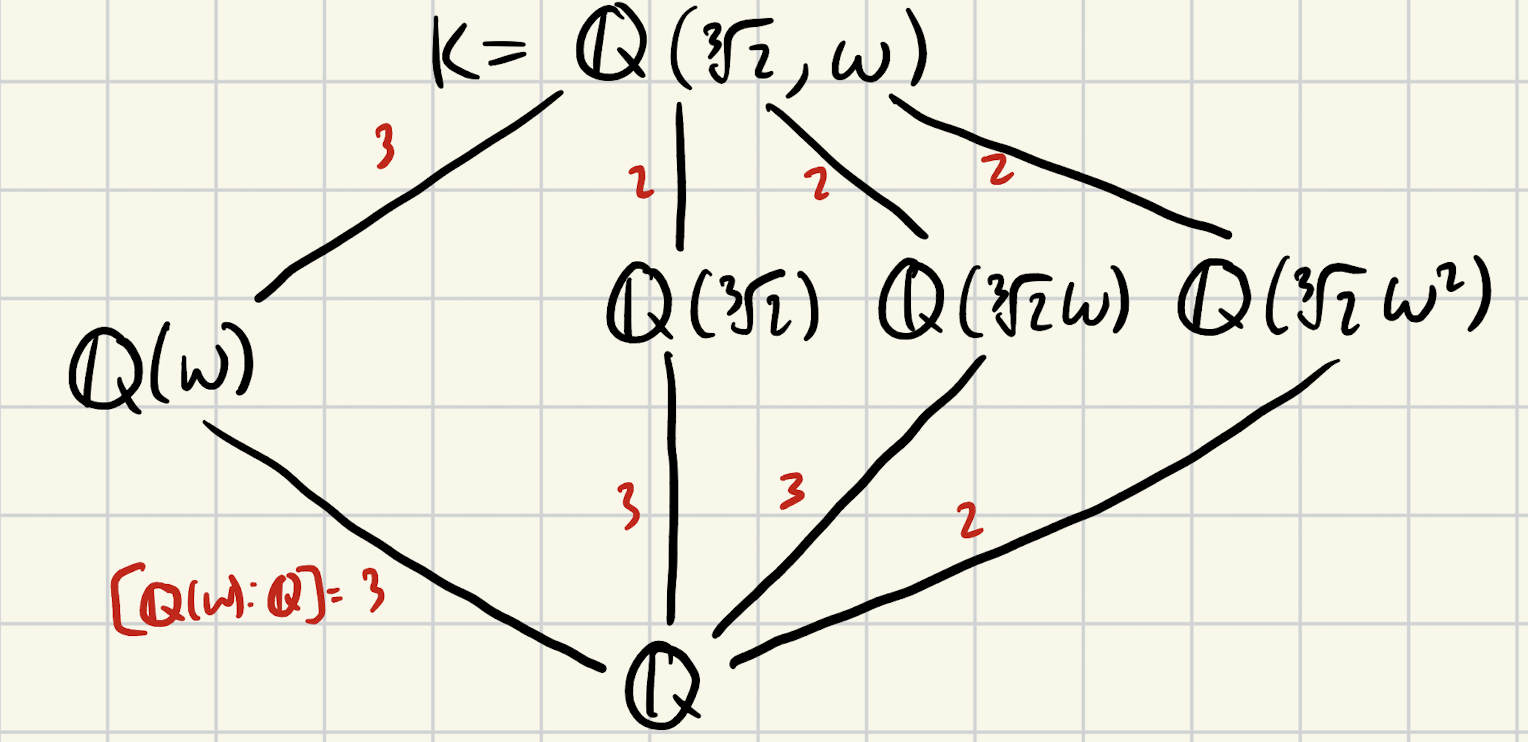
\includegraphics[width=350pt, center]{CH5/images/Subfield Lattice 1.png}

The subgroup lattice of the Galois group $K$ over $\Q$:

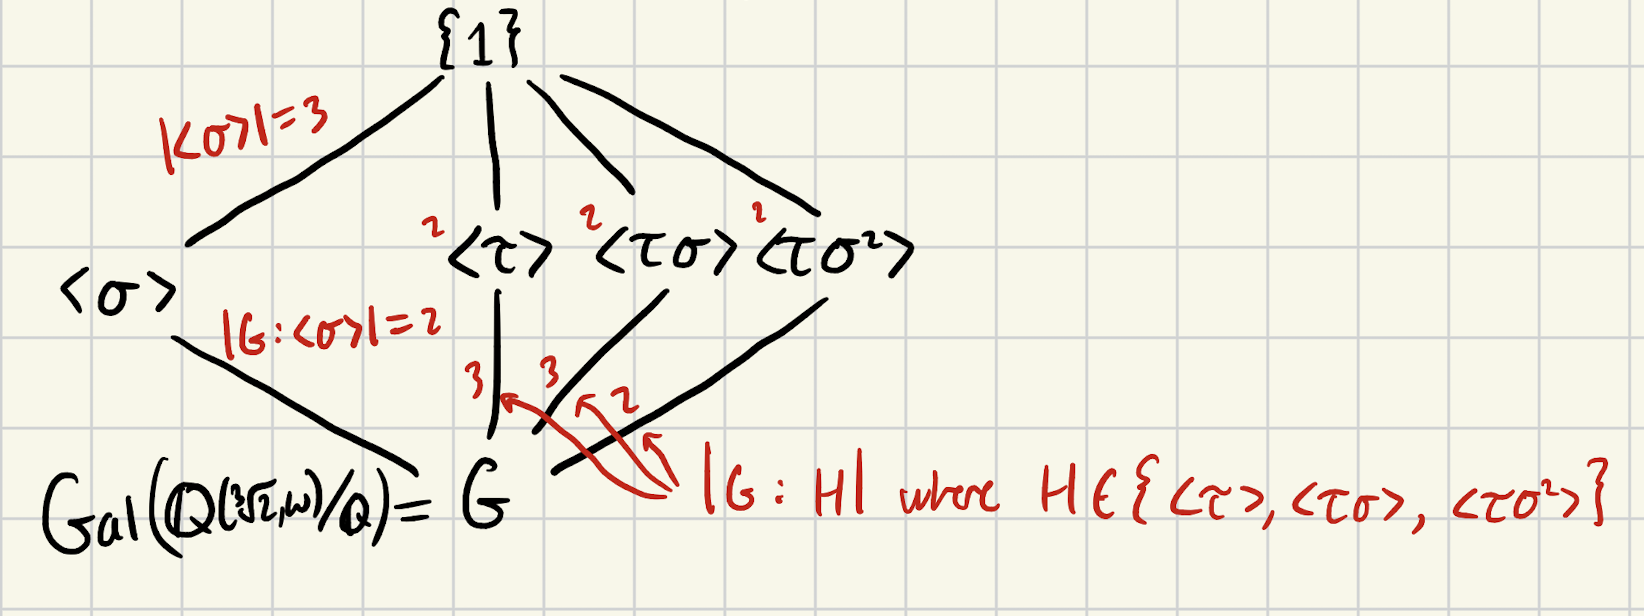
\includegraphics[width=350pt, center]{CH5/images/Subgroup Lattice 1.png}

\begin{theorem}[The Fundamental Theorem of Galois Theory] \leavevmode \\
    Let $K/F$ be a Galois extension and set $G = \Gal{K/F}$. Then there is a bijection between the set of subfields $E$ of $K$ containing $F$ and the subgroups of $G$
    $$
        \begin{tikzcd}[column sep=small]
            K \arrow[d, dash] \\
            E \arrow[d, dash] \\
            F
        \end{tikzcd}
        \longleftrightarrow
        \begin{tikzcd}[column sep=small]
            1 \arrow[d, dash] \\
            H \arrow[d, dash] \\
            G
        \end{tikzcd}
    $$
    given by the correspondence
    \begin{align*}
        E &\rightarrow \set{\text{the elements of $G$ fixing $E$}} \\
        \set{\text{The fixed field of $H$}} &\leftarrow H
    \end{align*}
    which are inverses to each other. Under this correspondence, we have the following results:
    \begin{enumerate}
        \item (Inclusion Reversing) If $E_1, E_2$ correspond to $H_1$ and $H_2$, respectively, then
        $$E_1 \subseteq E_2 \iff H_2 \subseteq H_1$$
        \item $[K:E] = |H|$ and $[E:F] = |G:H|$
        $$
        \begin{tikzcd}[column sep=large, row sep=large]
            K \arrow[d, dash, "\left. \rule{0pt}{2.5ex} \right\} |H|" right] \\
            E \arrow[d, dash, "\left. \rule{0pt}{2.5ex} \right\} |G:H|" right] \\
            F
        \end{tikzcd}
        $$
        \item The extension $K/E$ is always Galois with $\Gal{K/E}=H$.
        $$
        \begin{tikzcd}[column sep=large, row sep=large]
            K \arrow[d, dash, "\textstyle \quad H" right] \\
            E
        \end{tikzcd}
        $$
        \item $E$ is Galois over $F$ if and only if $H$ is a normal subroup of $G$. If this is the case, then the Galois group of $E$ over $F$ is isomorphic to the quotient group $\quotient{G}{H}$. That is,
        $$\Gal{E/F} \cong \quotient{G}{H}$$
        \item If $E_1, E_2$ correspond to $H_1, H_2,$ respectively, then $E_1 \cap E_2$ corresponds to the group $\cyc{H_1, H_2}$ and $E_1E_2$ corresponds to $H_1 \cap H_2$.
    \end{enumerate}
\end{theorem}

\begin{example}
    Let $p(x) = x^8-2$. Find the Galois group of the splitting field of $p(x)$ over $\Q$. The zeros of $p(x)$ are:
    $$\theta, \theta \zeta, \theta \zeta^2, \theta \zeta^3, ..., \theta \zeta^7 \text{ where } \zeta = \zeta_8, ~~ \theta = \sqrt[8]{2}$$
    Hence, $\theta, \theta \zeta \in K.$ Thus
    \begin{align*}
        \zeta = \dfrac{\theta \zeta}{\theta} &\in K \\
        \implies \Q(\theta, \zeta) &\subseteq K
    \end{align*}
    Further, each root of $p(x)$ can be constructed with $\theta$ and $\zeta$. Hence, $\theta \zeta^n \in \Q(\theta, \zeta)$ for all $n=0,1,..., 7.$ This gives $K \subseteq \Q(\theta, \zeta)$. Hence, $K = \Q(\theta, \zeta)$. We know $\zeta = \frac{1}{\sqrt{2}} + \frac{1}{\sqrt{2}}i,$ thus
    \begin{align*}
        \Q(\zeta) = \Q(i, \sqrt{2}) \\ 
        \left(\zeta + \zeta^7 = \sqrt{2}, ~~\zeta^2 = i\right)
    \end{align*}
    So, $K=\Q(\theta, i, \sqrt{2})$. But $\theta^4 = \sqrt{2}$, so $K = \Q(\theta, i)$ since $x^8-2$ is irreducible over $\Q$ by Eisenstein's. We have
    $$[\Q(\theta) : \Q] = 8$$
    and since $x^2+1$ is irreducible over $\Q$ with roots $\pm i$
    $$[\Q(i) : \Q] = 2$$
    so
    \begin{align*}
        [K : \Q] &\leq 2 \cdot 8 = 16 \\
        [K : \Q] &= [K : \Q(\theta)][\Q(\theta) : \Q]
    \end{align*}
    However, $K \neq \Q(\theta)$ since $\Q(\theta) \subseteq \R$ but $i \not \in \R$. Thus
    $$[K : \Q(\theta)] = 2$$
    It follows that $[K : \Q] = 16.$ Thus $G = \Gal{K/\Q}$ has order $16$. The possible automorphisms are
    $$\begin{cases*}
        \theta \mapsto \theta \zeta^a \\
        i \mapsto \pm i
    \end{cases*} \text{ where } a = 0,1,..., 7$$
    Define
    \begin{align*}
        \sigma: &\begin{cases*}
            \theta \mapsto \theta \zeta \\
            i \mapsto i
        \end{cases*} &&
        \tau: \begin{cases*}
            \theta \mapsto \theta \\
            i \mapsto -i
        \end{cases*} \\
        &(\zeta \mapsto \zeta^5)
        &&(\zeta \mapsto \bar{\zeta} = \zeta^7)
        \tag{$*$} \\
        \sigma^2: &\begin{cases*}
            \theta \mapsto \sigma(\theta \zeta) = \theta \zeta \cdot \theta^5 = \theta \zeta^6 \\
            i \mapsto i
        \end{cases*} \\
        &\vdots
    \end{align*}
    Continuing, we get $|\sigma| = 8$ and $|\tau| = 2.$ The group is 
    $$\set{1, \sigma, \sigma^2, ..., \sigma^7, \tau, \tau \sigma, ..., \tau \sigma^7}$$
    with $\sigma \tau = \tau \sigma^3.$ Thus
    $$G = \cyc{\tau, \sigma : \tau^2 = \sigma^8 = 1, \sigma \tau = \tau \sigma^3}$$
    This is a quasi-dihedral group.

    ($*$) Notice 
    \begin{align*}
        \sigma(\sqrt{2}) &= \sigma(\theta^4) \\
        &= \sigma(\theta)^4 \\
        &= \left(\theta \zeta\right)^4 \\
        &= \theta^4 \zeta^4 \\
        &= \theta^4(-1) \\
        &= -\sqrt{2}
    \end{align*} and so 
    \begin{align*}
        \zeta = \dfrac{1+i}{\sqrt{2}}, ~~\sigma(\zeta) = \dfrac{1+i}{-\sqrt{2}} = -\zeta = \zeta^5
    \end{align*}
\end{example}